\documentclass{beamer}

% Top-aligning columns within a top-aligned frame
% https://tex.stackexchange.com/questions/16447/beamer-top-aligning-columns-within-a-top-aligned-frame
\makeatletter
\newenvironment{myitemize}{%
   \setlength{\topsep}{0pt}
   \setlength{\partopsep}{0pt}
   \renewcommand*{\@listi}{\leftmargin\leftmargini \parsep\z@ \topsep\z@ \itemsep\z@}
   \let\@listI\@listi
   \itemize
}{\enditemize}
\makeatother  

\usepackage[USenglish]{babel}
\usepackage[utf8]{inputenc}
\usepackage{amssymb, amsmath}
\usepackage{bm}
\usepackage{color}
\usepackage{tikz}
\usepackage{url}

\definecolor{links}{HTML}{2A1B81}
\hypersetup{colorlinks,linkcolor=,urlcolor=links}

\usetheme{Boadilla}

\bibliographystyle{apalike}
% make bibliography entries smaller
%\renewcommand\bibfont{\scriptsize}
% Now get rid of all the colours
\setbeamercolor*{bibliography entry title}{fg=black}
\setbeamercolor*{bibliography entry author}{fg=black}
\setbeamercolor*{bibliography entry location}{fg=black}
\setbeamercolor*{bibliography entry note}{fg=black}

\newcommand{\lnorm}[1]{\left\lVert#1\right\rVert^2}
\newcommand{\norm}[1]{\left\lVert#1\right\rVert}

% and kill the abominable icon
\setbeamertemplate{bibliography item}{}

\begin{document}
\title[Distance Metrics with Proxies]{No Fuss Distance Metric Learning using Proxies}  
\author{Radek Bartyzal}
\date{14. 2. 2020} 
\institute{GLAMI AI}

\frame{\titlepage} 

\begin{frame}{Goal}

We have:
\begin{itemize}
\item dataset of products with multiple images per product
\end{itemize}

\vfill

We want:
\begin{itemize}
\item create embeddings of each product image 
\item embeddings of the same product images are closer to each other than to the embedding of images of the other products
\end{itemize}

\end{frame}

%--------- END Frame 12 -------------
\begin{frame}{Distance Metric Learning}

\begin{itemize}
\item learning a distance consistent with a notion of semantic similarity
\item an anchor point x is similar to
a set of positive points Y, and dissimilar to a set of negative
points Z
\item a loss defined over these distances is minimized 
\end{itemize}

\end{frame}

%--------- END Frame 12 -------------
\begin{frame}{Classic approaches}

\textbf{Triplet Ranking Loss}
\begin{itemize}
\item sample 1 anchor, 1 positive, 1 negative point = a triplet
\item optimize the 3 embeddings to:
\begin{itemize}
\item enlarge the distance between the anchor and negative point
\item shrink the distance between the anchor and positive point
\end{itemize}
\end{itemize}

\vfill

\textbf{Contrastive Loss (Pairwise Ranking Loss)}
\begin{itemize}
\item sample 1 anchor and 1 positive OR 1 negative point = a pair
\item optimize the 2 embeddings with the same goal as the triplet
\end{itemize}

\end{frame}

%--------- END Frame 12 -------------
\begin{frame}{Classic approaches}

\textbf{Triplet Ranking Loss:}
$$
L(x,y,z) = max(0,m + d(x,y) - d(x,z))
$$ \cite{cit:blog}

\vfill

\textbf{Contrastive Loss (Pairwise Ranking Loss):}
$$
L(x, y) = \left\{\begin{matrix} & d(x,y) & & if & PositivePair \\ & max(0, m - d(x,y)) & & if & NegativePair \end{matrix}\right.
$$ \cite{cit:blog}

$m$ = margin used to ignore triplets that have good enough embeddings
\end{frame}

%--------- END Frame 12 -------------
\begin{frame}{Problems}

Problem: 
\begin{itemize}
\item There are too many triplets to go through.
\end{itemize}

\vfill

Solution:
\begin{itemize}
\item we need to select \textbf{informative triplets} that will guide the optimization
\item informative triplets = not too easy, not too hard $=>$ \textbf{Semi-Hard negative mining} = select the right triplets from the mini-batch \cite{cit:semi-hard}
\item downside: requires large mini-batches (1800 images)
\item other approaches incorporating information outside the single triplet improve the convergence at the cost additional computation 
\end{itemize}

\end{frame}

%--------- END Frame 12 -------------
\begin{frame}{Approach with proxy embeddings}

\begin{itemize}
\item create a proxy embedding for each product = class
\item optimize distance to the proxy embeddings = proxies
\item optimize the proxies end-to-end with all the embeddings \cite{cit:metric}
\end{itemize}

\end{frame}

%--------- END Frame 12 -------------
\begin{frame}{Approach with proxy embeddings}

\begin{figure}[h]
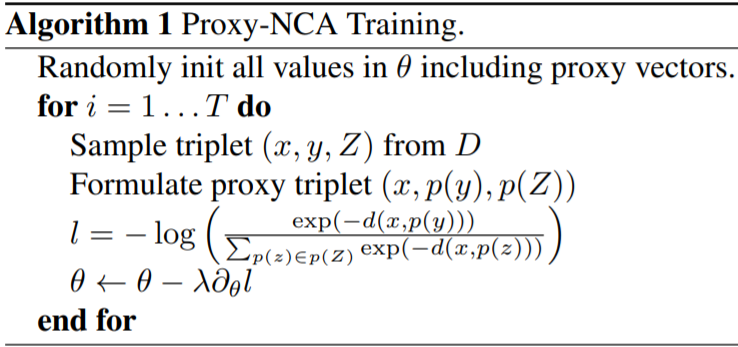
\includegraphics[width=\textwidth]{img/alg1}
\caption{Still have to sample the triplets, which is what we want to avoid.}
\end{figure}

\end{frame}

%--------- END Frame 12 -------------
\begin{frame}{One proxy embedding per class}

\begin{figure}[h]
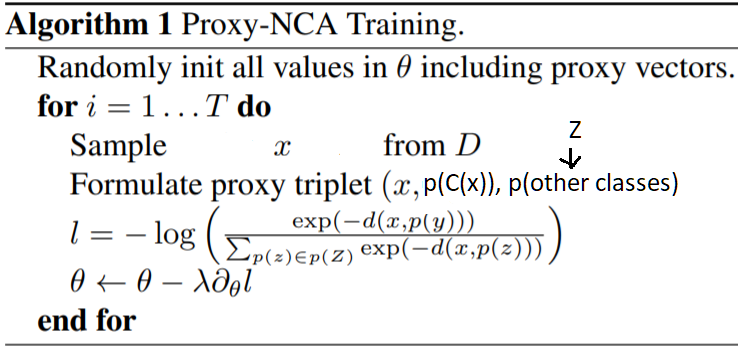
\includegraphics[width=\textwidth]{img/alg1_mine}
\caption{Optimization: sample the negative classes. \cite{cit:subsample}}
\end{figure}

\end{frame}

%--------- END Frame 12 -------------

\begin{frame}{Sources}

\begin{thebibliography}{0}

  \bibitem[1]{cit:metric} 1. Movshovitz-Attias, Yair, et al. "No fuss distance metric learning using proxies." Proceedings of the IEEE International Conference on Computer Vision. 2017. \url{https://arxiv.org/abs/1703.07464} 
  
  \bibitem[2]{cit:subsample} 2. Zhai, Andrew, and Hao-Yu Wu. "Classification is a Strong Baseline for Deep Metric Learning." arXiv preprint arXiv:1811.12649 (2018). \url{https://arxiv.org/abs/1811.12649}
  
  \bibitem[3]{cit:pint} 3. Zhai, Andrew, et al. "Learning a Unified Embedding for Visual Search at Pinterest." Proceedings of the 25th ACM SIGKDD International Conference on Knowledge Discovery \& Data Mining. 2019. \url{https://arxiv.org/abs/1908.01707}
  
  \bibitem[4]{cit:blog} 4. Blog: Understanding Ranking Loss, Contrastive Loss, Margin Loss, Triplet Loss, Hinge Loss and all those confusing names \url{https://gombru.github.io/2019/04/03/ranking_loss/}
  
\end{thebibliography}

\end{frame}

\begin{frame}{Sources}

\begin{thebibliography}{0}

  \bibitem[5]{cit:semi-hard} 5. Schroff, Florian, Dmitry Kalenichenko, and James Philbin. "Facenet: A unified embedding for face recognition and clustering." Proceedings of the IEEE conference on computer vision and pattern recognition. 2015. \url{https://www.cv-foundation.org/openaccess/content_cvpr_2015/papers/Schroff_FaceNet_A_Unified_2015_CVPR_paper.pdf} 

  
\end{thebibliography}

\end{frame}
 
\end{document}
